\documentclass[11pt]{article}

\usepackage{url}
\usepackage{multicol}
\usepackage[english]{babel}
\usepackage[margin=1in]{geometry}
\usepackage{graphicx}
\usepackage{subcaption}
\usepackage{enumitem}
\usepackage{amsmath}
\usepackage{amssymb}
\usepackage{wasysym}
\usepackage{color}
\usepackage{float}
\usepackage{nomencl}
\usepackage[title]{appendix}
\makenomenclature
\usepackage{pdfpages}
\usepackage{algorithm}
\usepackage{algpseudocode}
\usepackage{hyperref}
\hypersetup{
    colorlinks=true,
    linkcolor=blue,
    filecolor=magenta,      
    urlcolor=cyan,
    pdftitle={Overleaf Example},
    pdfpagemode=FullScreen,
    }
\title{16-745 Optimal Control Lecture 9}
\author{Reid Graves} 

\begin{document}
\maketitle

\section{Last time}
\begin{itemize}
    \item LQR via Shooting
    \item LQR as a QP
    \item LQR via Riccati
    \item Infinite Horizon LQR
\end{itemize}


\section{Today}
\begin{itemize}
    \item Controllability
    \item Dynamic Programming
\end{itemize}

\section{Controllability}
\begin{itemize}
    \item How do we know if LQR will work?
    \item We already know $Q\geq 0$, $R>0$
    \item For the time-invariant case there is a simple answer
    \item For any initial state $x_0$, $x_N$ is given by:
    \begin{align*}
        x_n &= Ax_{n-1} + Bu_{n-1}
        \\
        &= A(A_{x_{n-2} + Bu_{n-2}} + Bu_{n-1}
        \\
        \vdots
        \\
        &= A^Nx_0 + A^{N-1}Bu_0 + A^{n-2}Bu_1 + Bu_{N-1}
        \\
        &= \begin{bmatrix}
            B & AB & \dots & A^{N-1}B
        \end{bmatrix}
        \begin{bmatrix}
            u_{N-1} \\
            u_{N-2} \\
            u_{N-3}\\
            \vdots \\
            u_0
        \end{bmatrix}
        + A^Nx_0
    \end{align*}
    \item $\begin{bmatrix}
            B & AB & \dots & A^{N-1}B
        \end{bmatrix}$ is $C$
    \item Without loss of generality, we solve for $x_N=0$
    \item This is equivalent to a least-squares problem for $u_{0:N-1}$:
    \begin{align*}
        \begin{bmatrix}
            u_{N-1}\\
            u_{N-2}\\
            \vdots \\
            u_0
        \end{bmatrix}
        &=
        \begin{bmatrix}
            C^T(CC^T)^{-1}
        \end{bmatrix}(x_N - A^N)x_0
    \end{align*}
    \item $C^T(CC^T)^{-1}$ is the ``pseudo-inverse":
    \item For $CC^T$ to be invertable: 
    \begin{align*}
        \Rightarrow rank(C) &= n, \quad n=dim(x)
    \end{align*}
    \item I can stop at $n$ time steps in $C$ because the Cayley-Hamilton theorem says that ``$A^N$" can be written in terms of a linear combination of lower powers of $A$ up to $N$
    \begin{align*}
        A^N &= \sum_{k=0}^{N-1}\alpha_kA^k \quad\text{(for some } \alpha_k)
    \end{align*}
    \item therefore adding more time steps/columns to C can't increase the rank:
    \begin{align*}
        \Rightarrow C &= \begin{bmatrix}
            B & AB & \dots & A^{N-1}B
        \end{bmatrix}\quad \text{``Controllability Matrix"}
    \end{align*}
\end{itemize}


\section{Bellman's Principle}
\begin{itemize}
    \item Optimal control problems have an inherently sequential structure
    \item Past control inputs can only affect future states. Future inputs can't affect past states.
    \item Bellman's Principle (``Princible of Optimality") formulates this
    % insert figure here
    \begin{figure}[H]
        \centering
        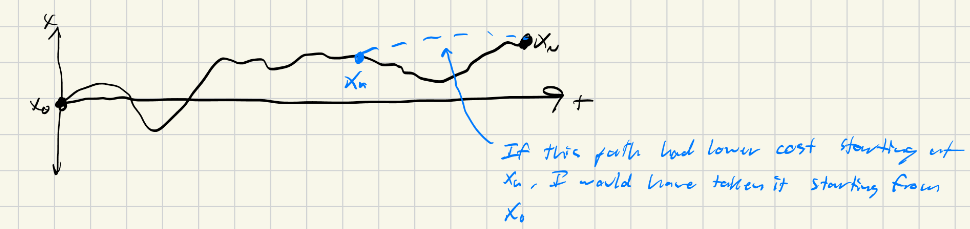
\includegraphics[width=0.9\linewidth]{l9_1.png}
    \end{figure}
    \item Sub trajectories of optimal trajectories have to be optimal for the appropriately defined sub problem.
\end{itemize}

\subsection{Dynamic Programming}
\begin{itemize}
    \item Bellman's Principle suggests starting from the end of the trajectory and working backwards. 
    \item We've already seen this with Riccati and Pontryagin
    \item Define ``Optimal cost to go" aka ``Value function" $V_k(x)$
    \item Encodes cost incurred starting from state $x$ at time $k$ if we act optimally
    \item For LQR
    \begin{align*}
        V_N(x) &= \frac{1}{2}x^TQ_Nx = \frac{1}{2}x^TP_Nx
    \end{align*}
    \item Back up one step and calculate $V_{N-1}(x)$:
    \begin{align*}
        V_{N-1} &= \min_u \frac{1}{2}x_{N-1}^TQx_{N-1} + \frac{1}{2}u^TRu + V_N(Ax_{N-1}+Bu_{N-1})
    \end{align*}
    We want to minimize for the control input $u_{N-1}$. Substituting in our value for $V_N$:
    \begin{align*}
        &\Rightarrow \min_u \frac{1}{2}u^TRu+\frac{1}{2}(Ax_{N-1}+Bu)^TP_N(Ax_{N-1}+Bu)
        \\
        &\text{Taking the gradient and setting to 0:}
        \\
        &\Rightarrow Ru + B^TP_N(Ax_{N-1}+Bu) = 0
        \\
        &\text{Then solving for }u_{N-1}:
        \\
        &\Rightarrow u_{N-1} = -(R+B^TP_NB)^{-1}BP_NAx_{N-1}\quad \text{term before } x_{N-1} \text{is }(K_{N-1})
    \end{align*}
    \item Plug $u=-Kx$ back into 
    \begin{align*}
        &\Rightarrow V_{N-1}(x) = \frac{1}{2}x^T\begin{bmatrix}
            Q + K^TRK + (A-BK)^TP_N(A-BK)
        \end{bmatrix}x \quad 
        \\
        &P_{N-1} = \begin{bmatrix}
            Q + K^TRK + (A-BK)^TP_N(A-BK)
        \end{bmatrix}
        \\
        &\Rightarrow V_{N-1}(x) = \frac{1}{2}x^TP_{N-1}x
    \end{align*}
    \item Now we have a backward recursion for $K$ and $P$ that we iterate until $K=0$
\end{itemize}
\subsection{Dynamic Programming Algorithm}
\begin{align*}
    &V_N(x)\leftarrow l_N(x)
    \\
    k &\leftarrow N
    \\
    &\text{while } k>1
    \\
    &\quad V_{k-1}(x) = \min_{u\in \mathcal{U}}\begin{bmatrix}
        l(x,u) + V_k(f(x,u)
    \end{bmatrix}
    \\
    k&\leftarrow k-1
    \\
    \text{end}
\end{align*}
\begin{itemize}
    \item If we know $V_k(x)$, the optimal policy is: 
    \begin{align*}
        u_k(x) = \text{arg}\min_{u\in\mathcal{U}}\begin{bmatrix}
            l(x,u) + V_{k+1}(f(x,u))
        \end{bmatrix}
    \end{align*}
    \item DP equations can be written equivalently written in terms of ``action-value" or ``Q" function:
    \begin{align*}
        S_k(x,u) &=l(x,u) + V_{k+1}(f(x,u))
    \end{align*}
    \item Usually denoted $Q(x,u)$, but we'll use $S(x,u)$
    \item Avoids need for explicit dynamics model
\end{itemize}

\subsection{The curse of dimensionality}
\begin{itemize}
    \item DP is sufficient for global optimum
    \item Only tractable for simple problems (LQR, low dimensional)
    \item $V(x)$ stays quadratic for LQR but becomes impossible to write analytically, even for simple nonlinear problems
    \item Even if we could, $\min_u S(x,u)$ will be non-convex and possibly hard to solve
    \item Cost of DP blows up with state dimension due to cost of representing $V(x)$
\end{itemize}
\subsection{Why do we care?}
\begin{itemize}
    \item Approximate DP with a function approximator for $V(x)$ or $S(x,u)$ is very powerful
    \item Forms basis for modern RL
    \item DP generalizes to stochastic problem (Just wrap everything in expectations). Pontryagin does not.
\end{itemize}

\subsection{Finally: What are the Lagrange Multipliers?}
\begin{itemize}
    \item Recall Ricatti derivation from QP:
    \begin{align*}
        \lambda_k &= p_kx_k
    \end{align*}
    \item From Dynamic Programing:
    \begin{align*}
        V(x) &= \frac{1}{2}x^TPx
        \\
        \Rightarrow \lambda_k &= \nabla_x V_k(x)
    \end{align*}
    \item Dynamics multipliers are cost-to-go gradients
    \item Carries over to nonlinear setting (Not just LQR)
\end{itemize}

\end{document}
